% Final Figure 1, one two-column float at the TOP of page 2.
% Insert exactly once via % Final Figure 1, one two-column float at the TOP of page 2.
% Insert exactly once via % Final Figure 1, one two-column float at the TOP of page 2.
% Insert exactly once via % Final Figure 1, one two-column float at the TOP of page 2.
% Insert exactly once via \input{fig/fig1_page2} directly after
% \section{Introduction}\label{sec:intro}.
% Do not also include the official \input{fig/teaser} in main.tex.
% Do not use strip, captionof, clearpage, afterpage or negative vspace.
\begin{figure*}[t]
  \centering
  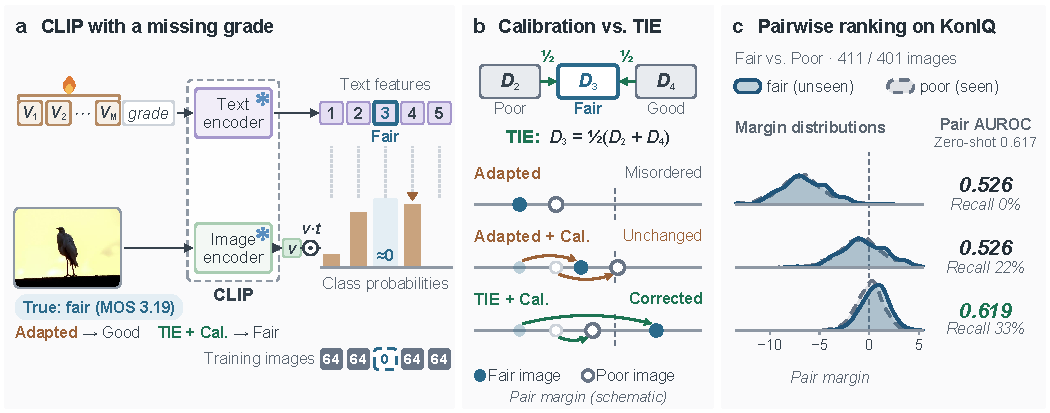
\includegraphics[width=\textwidth]{figures/fig1.pdf}
  \caption{\textbf{Fixing the score is not fixing the order.}
  (a) CLIP adaptation with a missing grade, illustrated with a CoOp-style adapter ($M=4$ learned context tokens; frozen encoders) on KonIQ grades, i.e., MOS quintiles prompted as \emph{bad}, \emph{poor}, \emph{fair}, \emph{good}, \emph{excellent}. Adaptation uses no grade-3 (fair) images. For this grade-3 photo (MOS 3.19), the adapted probability of grade 3 is 0.008\% and the model predicts grade 4 (good); TIE + Cal. predicts grade 3.
  (b) Post-hoc class-bias calibration adds one constant to the missing grade's score, so every image moves by the same amount along the pairwise score margin and their order cannot change (Prop.~1). TIE ties the missing grade to its nearest seen grades: image by image, its reference-relative score displacement $D=S-T$ becomes the mean of theirs ($T$: zero-shot CLIP with the prompt ``a photograph with \{grade\} image quality.''); schematic.
  (c) Pairwise score margin between grade 3 (fair) and grade 2 (poor) for all 411 and 401 test images (seed 101; Gaussian kernel, bandwidth 0.45). Adaptation lowers the pair AUROC from 0.617 (zero-shot CLIP) to 0.526. Calibration ($c^*=6$) raises the five-way grade-3 recall from 0\% to 22\% and leaves the pair AUROC unchanged; TIE + Cal. ($c^*=0$) raises it to 0.619, with 33\% recall.}
  \label{fig:teaser}
\end{figure*}

 directly after
% \section{Introduction}\label{sec:intro}.
% Do not also include the official \input{fig/teaser} in main.tex.
% Do not use strip, captionof, clearpage, afterpage or negative vspace.
\begin{figure*}[t]
  \centering
  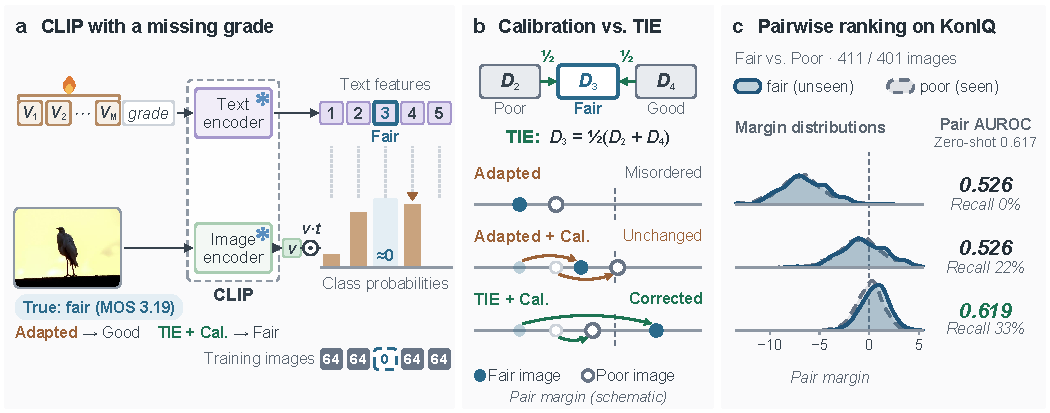
\includegraphics[width=\textwidth]{figures/fig1.pdf}
  \caption{\textbf{Fixing the score is not fixing the order.}
  (a) CLIP adaptation with a missing grade, illustrated with a CoOp-style adapter ($M=4$ learned context tokens; frozen encoders) on KonIQ grades, i.e., MOS quintiles prompted as \emph{bad}, \emph{poor}, \emph{fair}, \emph{good}, \emph{excellent}. Adaptation uses no grade-3 (fair) images. For this grade-3 photo (MOS 3.19), the adapted probability of grade 3 is 0.008\% and the model predicts grade 4 (good); TIE + Cal. predicts grade 3.
  (b) Post-hoc class-bias calibration adds one constant to the missing grade's score, so every image moves by the same amount along the pairwise score margin and their order cannot change (Prop.~1). TIE ties the missing grade to its nearest seen grades: image by image, its reference-relative score displacement $D=S-T$ becomes the mean of theirs ($T$: zero-shot CLIP with the prompt ``a photograph with \{grade\} image quality.''); schematic.
  (c) Pairwise score margin between grade 3 (fair) and grade 2 (poor) for all 411 and 401 test images (seed 101; Gaussian kernel, bandwidth 0.45). Adaptation lowers the pair AUROC from 0.617 (zero-shot CLIP) to 0.526. Calibration ($c^*=6$) raises the five-way grade-3 recall from 0\% to 22\% and leaves the pair AUROC unchanged; TIE + Cal. ($c^*=0$) raises it to 0.619, with 33\% recall.}
  \label{fig:teaser}
\end{figure*}

 directly after
% \section{Introduction}\label{sec:intro}.
% Do not also include the official \input{fig/teaser} in main.tex.
% Do not use strip, captionof, clearpage, afterpage or negative vspace.
\begin{figure*}[t]
  \centering
  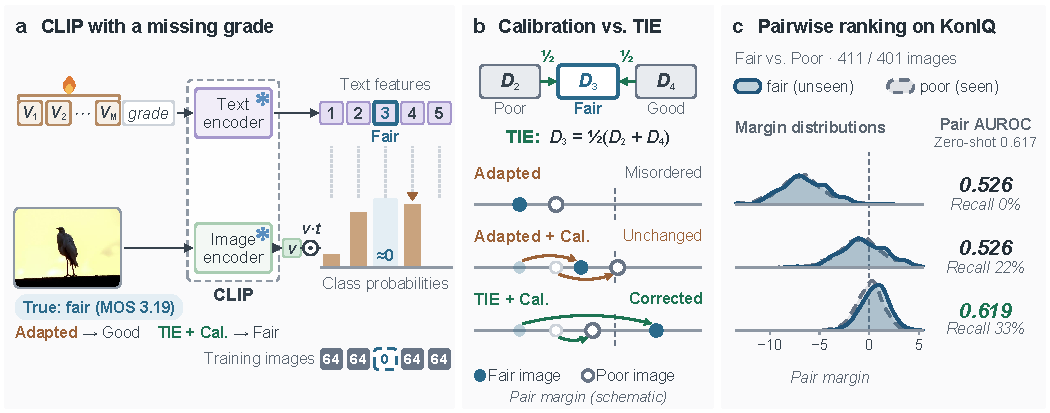
\includegraphics[width=\textwidth]{figures/fig1.pdf}
  \caption{\textbf{Fixing the score is not fixing the order.}
  (a) CLIP adaptation with a missing grade, illustrated with a CoOp-style adapter ($M=4$ learned context tokens; frozen encoders) on KonIQ grades, i.e., MOS quintiles prompted as \emph{bad}, \emph{poor}, \emph{fair}, \emph{good}, \emph{excellent}. Adaptation uses no grade-3 (fair) images. For this grade-3 photo (MOS 3.19), the adapted probability of grade 3 is 0.008\% and the model predicts grade 4 (good); TIE + Cal. predicts grade 3.
  (b) Post-hoc class-bias calibration adds one constant to the missing grade's score, so every image moves by the same amount along the pairwise score margin and their order cannot change (Prop.~1). TIE ties the missing grade to its nearest seen grades: image by image, its reference-relative score displacement $D=S-T$ becomes the mean of theirs ($T$: zero-shot CLIP with the prompt ``a photograph with \{grade\} image quality.''); schematic.
  (c) Pairwise score margin between grade 3 (fair) and grade 2 (poor) for all 411 and 401 test images (seed 101; Gaussian kernel, bandwidth 0.45). Adaptation lowers the pair AUROC from 0.617 (zero-shot CLIP) to 0.526. Calibration ($c^*=6$) raises the five-way grade-3 recall from 0\% to 22\% and leaves the pair AUROC unchanged; TIE + Cal. ($c^*=0$) raises it to 0.619, with 33\% recall.}
  \label{fig:teaser}
\end{figure*}

 directly after
% \section{Introduction}\label{sec:intro}.
% Do not also include the official \input{fig/teaser} in main.tex.
% Do not use strip, captionof, clearpage, afterpage or negative vspace.
\begin{figure*}[t]
  \centering
  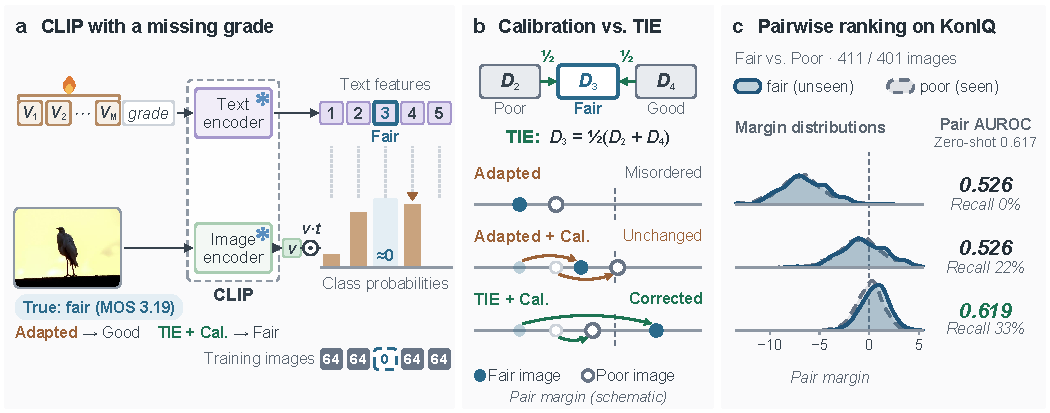
\includegraphics[width=\textwidth]{figures/fig1.pdf}
  \caption{\textbf{Fixing the score is not fixing the order.}
  (a) CLIP adaptation with a missing grade, illustrated with a CoOp-style adapter ($M=4$ learned context tokens; frozen encoders) on KonIQ grades, i.e., MOS quintiles prompted as \emph{bad}, \emph{poor}, \emph{fair}, \emph{good}, \emph{excellent}. Adaptation uses no grade-3 (fair) images. For this grade-3 photo (MOS 3.19), the adapted probability of grade 3 is 0.008\% and the model predicts grade 4 (good); TIE + Cal. predicts grade 3.
  (b) Post-hoc class-bias calibration adds one constant to the missing grade's score, so every image moves by the same amount along the pairwise score margin and their order cannot change (Prop.~1). TIE ties the missing grade to its nearest seen grades: image by image, its reference-relative score displacement $D=S-T$ becomes the mean of theirs ($T$: zero-shot CLIP with the prompt ``a photograph with \{grade\} image quality.''); schematic.
  (c) Pairwise score margin between grade 3 (fair) and grade 2 (poor) for all 411 and 401 test images (seed 101; Gaussian kernel, bandwidth 0.45). Adaptation lowers the pair AUROC from 0.617 (zero-shot CLIP) to 0.526. Calibration ($c^*=6$) raises the five-way grade-3 recall from 0\% to 22\% and leaves the pair AUROC unchanged; TIE + Cal. ($c^*=0$) raises it to 0.619, with 33\% recall.}
  \label{fig:teaser}
\end{figure*}

